\documentclass[margin=1mm]{standalone}
%
%\usepackage{amsmath,amssymb,latexsym,float,epsfig,hyperref}
%\usepackage{framed,color,url,fancybox,fullpage,booktabs,subfigure,wrapfig,chngpage,setspace}

\usepackage[latin1]{inputenc}
\usepackage{tikz}

\usetikzlibrary{shapes,arrows}
\usetikzlibrary{arrows,positioning,mindmap} 
\usetikzlibrary{calc,trees,positioning,arrows,chains,shapes.geometric,%
decorations.pathreplacing,decorations.pathmorphing,shapes,%
matrix,shapes.symbols,plotmarks,decorations.markings,shadows}
\usetikzlibrary{patterns}

\tikzstyle{decision} = [diamond, draw, fill=gray!10,
  text width=6em, text badly centered, node distance=2.5cm, 
  inner sep=0pt,minimum height=1em,text centered]
\tikzstyle{block} = [rectangle, draw, fill=blue!20,
  text width=10em, text centered, rounded corners, minimum height=3.0em]

\tikzstyle{autoblock} = [rectangle, draw, fill=blue!20, text centered, rounded corners]

\tikzstyle{cloud} = [draw, ellipse,fill={rgb:orange,1;yellow,1;pink,1}, node distance=4cm,
    minimum height=1em,text centered]
\tikzstyle{circ} = [draw,circle,fill={rgb:orange,1;yellow,1;pink,1}, 
  node distance=4cm, minimum height=2em, text centered]

\tikzstyle{line} = [draw, very thick, color=black!50, -latex']
\tikzstyle{redline} = [draw, very thick, color=black!50, -latex']
\tikzstyle{dotline} = [draw,dotted, very thick, color=black!50, -latex']

\tikzset{
    poly/.style={
        draw, 
        shape border rotate=0,
        regular polygon,
        regular polygon sides=3,
        fill=red,
        node distance=2cm,
        minimum height=4em, 
    }
}

\tikzstyle{line} = [draw, very thick, color=black, -latex']
\tikzstyle{redline} = [draw, very thick, color=red, -latex']
\tikzstyle{dotline} = [draw,dotted, very thick, color=black!50, -latex']


% find center of two nodes
% https://tex.stackexchange.com/questions/71478/how-to-center-one-node-exactly-between-two-others-with-tikz
\tikzset{
    between/.style args={#1 and #2}{
         at = ($(#1)!0.5!(#2)$)
    }
}

%\tikzset{
%between base/.style args={#1 and #2}{
%between=#1.base and #2.base
%}
%}


% https://tex.stackexchange.com/questions/72784/arrow-with-two-colors-with-tikz
\tikzset{
  double arrow/.style args={#1 colored by #2 and #3}{
    -stealth,line width=#1,#2, % first arrow
    postaction={draw,-stealth,#3,line width=(#1)/3,
                shorten <=(#1)/3,shorten >=2*(#1)/3}, % second arrow
  }
}

\tikzset{
  double -latex/.style args={#1 colored by #2 and #3}{    
    -latex,line width=#1,#2,
    postaction={draw,-latex,#3,line width=(#1)/3,shorten <=(#1)/4,shorten >=4.5*(#1)/3},
  },
  double round cap-latex/.style args={#1 colored by #2 and #3}{    
    round cap-latex,line width=#1,#2,
    postaction={draw,round cap-latex,#3,line width=(#1)/3,shorten <=(#1)/4,shorten >=4.5*(#1)/3},
  },
  double round cap-stealth/.style args={#1 colored by #2 and #3}{
    round cap-stealth,line width=#1,#2,
    postaction={round cap-stealth,draw,,#3,line width=(#1)/3,shorten <=(#1)/3,shorten >=2*(#1)/3},
  },
  double -stealth/.style args={#1 colored by #2 and #3}{
    -stealth,line width=#1,#2,
    postaction={-stealth,draw,,#3,line width=(#1)/3,shorten <=(#1)/3,shorten >=2*(#1)/3},
  },
}


\makeatletter 
\@namedef{color@1}{red!40}
\@namedef{color@2}{green!40}   
\@namedef{color@3}{blue!40} 
\@namedef{color@4}{cyan!40}  
\@namedef{color@5}{magenta!40} 
\@namedef{color@6}{yellow!40}    

\newcommand{\graphitemize}[2]{%
  \begin{tikzpicture}[at start, every node/.style={align=center}]  
    \node[minimum size=5cm,circle,
%    fill=gray!40,
ultra thick,
 fill = white,
 text  = black,
 draw = black,
    font=\Large, outer sep=1cm,inner sep=.5cm](ce){#1};  
    \foreach \gritem [count=\xi] in {#2}
             {\global\let\maxgritem\xi}  
             \foreach \gritem [count=\xi] in {#2}
                      {% 
                        \pgfmathtruncatemacro{\angle}{360/\maxgritem*\xi}
                        \edef\col{\@nameuse{color@\xi}}
                        \node[circle,
                        font=\bfseries\Large,    
                          ultra thick,
                          draw=white,
                          %                          fill opacity=.75,
                          fill = black,
                          text = white,
                          minimum size=3cm] at (ce.\angle) {\gritem };}%
  \end{tikzpicture}  
}%

\tikzset{
  ring shading/.code args={from #1 at #2 to #3 at #4}{
    \def\colin{#1}
    \def\radin{#2}
    \def\colout{#3}
    \def\radout{#4}
    \pgfmathsetmacro{\proportion}{\radin/\radout}
    \pgfmathsetmacro{\outer}{.8818cm}
    \pgfmathsetmacro{\inner}{.8818cm*\proportion}
    \pgfmathsetmacro{\innerlow}{\inner-0.01pt}
    \pgfdeclareradialshading{ring}{\pgfpoint{0cm}{0cm}}%
    {
      color(0pt)=(white);
      color(\innerlow)=(white);
      color(\inner)=(#1);
      color(\outer)=(#3)
    }
    \pgfkeysalso{/tikz/shading=ring}
  },
}


\usepackage[standard-baselineskips]{cmbright}
\renewcommand\familydefault{\sfdefault}
\usepackage[T1]{fontenc}

% % % \include{tableau_colors} in your .tex file to use these custom
% Tableau colors
% https://gist.github.com/AndiH/c957b4d769e628f506bd

\definecolor{dblue}{RGB}{31, 119, 180}
\definecolor{lblue}{RGB}{174, 199, 232}

\definecolor{dorange}{RGB}{255, 127, 14}
\definecolor{lorange}{RGB}{255, 187, 120}

\definecolor{dgreen}{RGB}{44, 160, 44}
\definecolor{lgreen}{RGB}{152, 223, 138}

\definecolor{dred}{RGB}{214, 39, 40}
\definecolor{lred}{RGB}{255, 152, 150}

\definecolor{dpurple}{RGB}{148, 103, 189} 
\definecolor{lpurple}{RGB}{197, 176, 213}

\definecolor{dbrown}{RGB}{140, 86, 75} 
\definecolor{lbrown}{RGB}{196, 156, 148}    

\definecolor{dpink}{RGB}{227, 119, 194}
\definecolor{lpink}{RGB}{247, 182, 210}

\definecolor{dgray}{RGB}{127, 127, 127}
\definecolor{lgray}{RGB}{199, 199, 199}

\definecolor{dolive}{RGB}{188, 189, 34}
\definecolor{lolive}{RGB}{219, 219, 141}

\definecolor{dskyblue}{RGB}{23, 190, 207}
\definecolor{lskyblue}{RGB}{158, 218, 229}

\definecolor{gold}{RGB}{255,223,0}
 in your .tex file to use these custom
% Tableau colors
% https://gist.github.com/AndiH/c957b4d769e628f506bd

\definecolor{dblue}{RGB}{31, 119, 180}
\definecolor{lblue}{RGB}{174, 199, 232}

\definecolor{dorange}{RGB}{255, 127, 14}
\definecolor{lorange}{RGB}{255, 187, 120}

\definecolor{dgreen}{RGB}{44, 160, 44}
\definecolor{lgreen}{RGB}{152, 223, 138}

\definecolor{dred}{RGB}{214, 39, 40}
\definecolor{lred}{RGB}{255, 152, 150}

\definecolor{dpurple}{RGB}{148, 103, 189} 
\definecolor{lpurple}{RGB}{197, 176, 213}

\definecolor{dbrown}{RGB}{140, 86, 75} 
\definecolor{lbrown}{RGB}{196, 156, 148}    

\definecolor{dpink}{RGB}{227, 119, 194}
\definecolor{lpink}{RGB}{247, 182, 210}

\definecolor{dgray}{RGB}{127, 127, 127}
\definecolor{lgray}{RGB}{199, 199, 199}

\definecolor{dolive}{RGB}{188, 189, 34}
\definecolor{lolive}{RGB}{219, 219, 141}

\definecolor{dskyblue}{RGB}{23, 190, 207}
\definecolor{lskyblue}{RGB}{158, 218, 229}

\definecolor{gold}{RGB}{255,223,0}
 in your .tex file to use these custom
% Tableau colors
% https://gist.github.com/AndiH/c957b4d769e628f506bd

\definecolor{dblue}{RGB}{31, 119, 180}
\definecolor{lblue}{RGB}{174, 199, 232}

\definecolor{dorange}{RGB}{255, 127, 14}
\definecolor{lorange}{RGB}{255, 187, 120}

\definecolor{dgreen}{RGB}{44, 160, 44}
\definecolor{lgreen}{RGB}{152, 223, 138}

\definecolor{dred}{RGB}{214, 39, 40}
\definecolor{lred}{RGB}{255, 152, 150}

\definecolor{dpurple}{RGB}{148, 103, 189} 
\definecolor{lpurple}{RGB}{197, 176, 213}

\definecolor{dbrown}{RGB}{140, 86, 75} 
\definecolor{lbrown}{RGB}{196, 156, 148}    

\definecolor{dpink}{RGB}{227, 119, 194}
\definecolor{lpink}{RGB}{247, 182, 210}

\definecolor{dgray}{RGB}{127, 127, 127}
\definecolor{lgray}{RGB}{199, 199, 199}

\definecolor{dolive}{RGB}{188, 189, 34}
\definecolor{lolive}{RGB}{219, 219, 141}

\definecolor{dskyblue}{RGB}{23, 190, 207}
\definecolor{lskyblue}{RGB}{158, 218, 229}

\definecolor{gold}{RGB}{255,223,0}

%
\usepackage{bm}
\usepackage{amsmath}
\usepackage{amssymb}
%
% Define inner product in latex
\newcommand\inner[2]{{\Bigg\langle} #1 ~\Bigg|~ #2 {\Bigg\rangle}}
\newcommand\sinner[2]{{\Big\langle} #1 ~\Big|~ #2 {\Big\rangle}}
\newcommand\linner[2]{{\big\langle} #1 ~\big|~ #2 {\big\rangle}}
\newcommand\oinner[2]{{\langle} #1 ~|~ #2 {\rangle}}
\newcommand\otinner[3]{{\langle} #1 |#2| #3 {\rangle}}
\newcommand\cinner[2]{{\langle} #1 | #2 {\rangle}}
\newcommand\crinner[2]{{(} #1 | #2 {)}}

% Define commands
\newcommand{\half}{\ensuremath{\frac{1}{2}}}

\newcommand{\bea}{\begin{eqnarray}}
\newcommand{\eea}{\end{eqnarray}}
\newcommand{\beq}{\begin{equation}}
\newcommand{\eeq}{\end{equation}}
\newcommand{\bed}{\begin{displaymath}}
\newcommand{\eed}{\end{displaymath}}

\newcommand{\pd}[2]{\dfrac{\partial #1}{\partial #2}}
\newcommand{\pf}[2]{\dfrac{d #1}{d #2}}
\newcommand{\pdt}[2]{\dfrac{\partial^2 #1}{\partial #2^2}}
\newcommand{\pft}[2]{\dfrac{d^2 #1}{d #2^2}}
\newcommand{\pdtno}[2]{\dfrac{\partial^2 #1}{\partial #2}}
\newcommand{\pdd}[3]{\dfrac{\partial^2 #1}{\partial #2 \partial #3}}
\newcommand{\pff}[3]{\dfrac{d^2 #1}{d #2 d #3}}
\newcommand{\tdt}[2]{\dfrac{d^2 #1}{d #2^2}}
\newcommand{\td}[2]{\dfrac{d #1}{d #2}}
\newcommand{\mb}{\bm}

\newcommand{\x}{\bm{x}}
\newcommand{\y}{\bm{y}}
\newcommand{\z}{\bm{z}}

\newcommand{\q}{\bm{q}}
\renewcommand{\u}{\bm{u}}
\renewcommand{\v}{\bm{v}}
\newcommand{\qd}{\bm{\dot{q}}}
\newcommand{\qdd}{\bm{\ddot{q}}}
\newcommand{\R}{\bm{R}}
\renewcommand{\S}{\bm{S}}
\newcommand{\zerovec}{\bm{0}}

\newcommand{\for}{\mathrm{for}}
\renewcommand{\arg}[1]{\textcolor{black!70}{(#1)}}
\newcommand{\sarg}[1]{\textcolor{black!70}{#1}}
\newcommand{\carg}[1]{\textcolor{black!70}{#1}}

\begin{document}
\thispagestyle{empty}

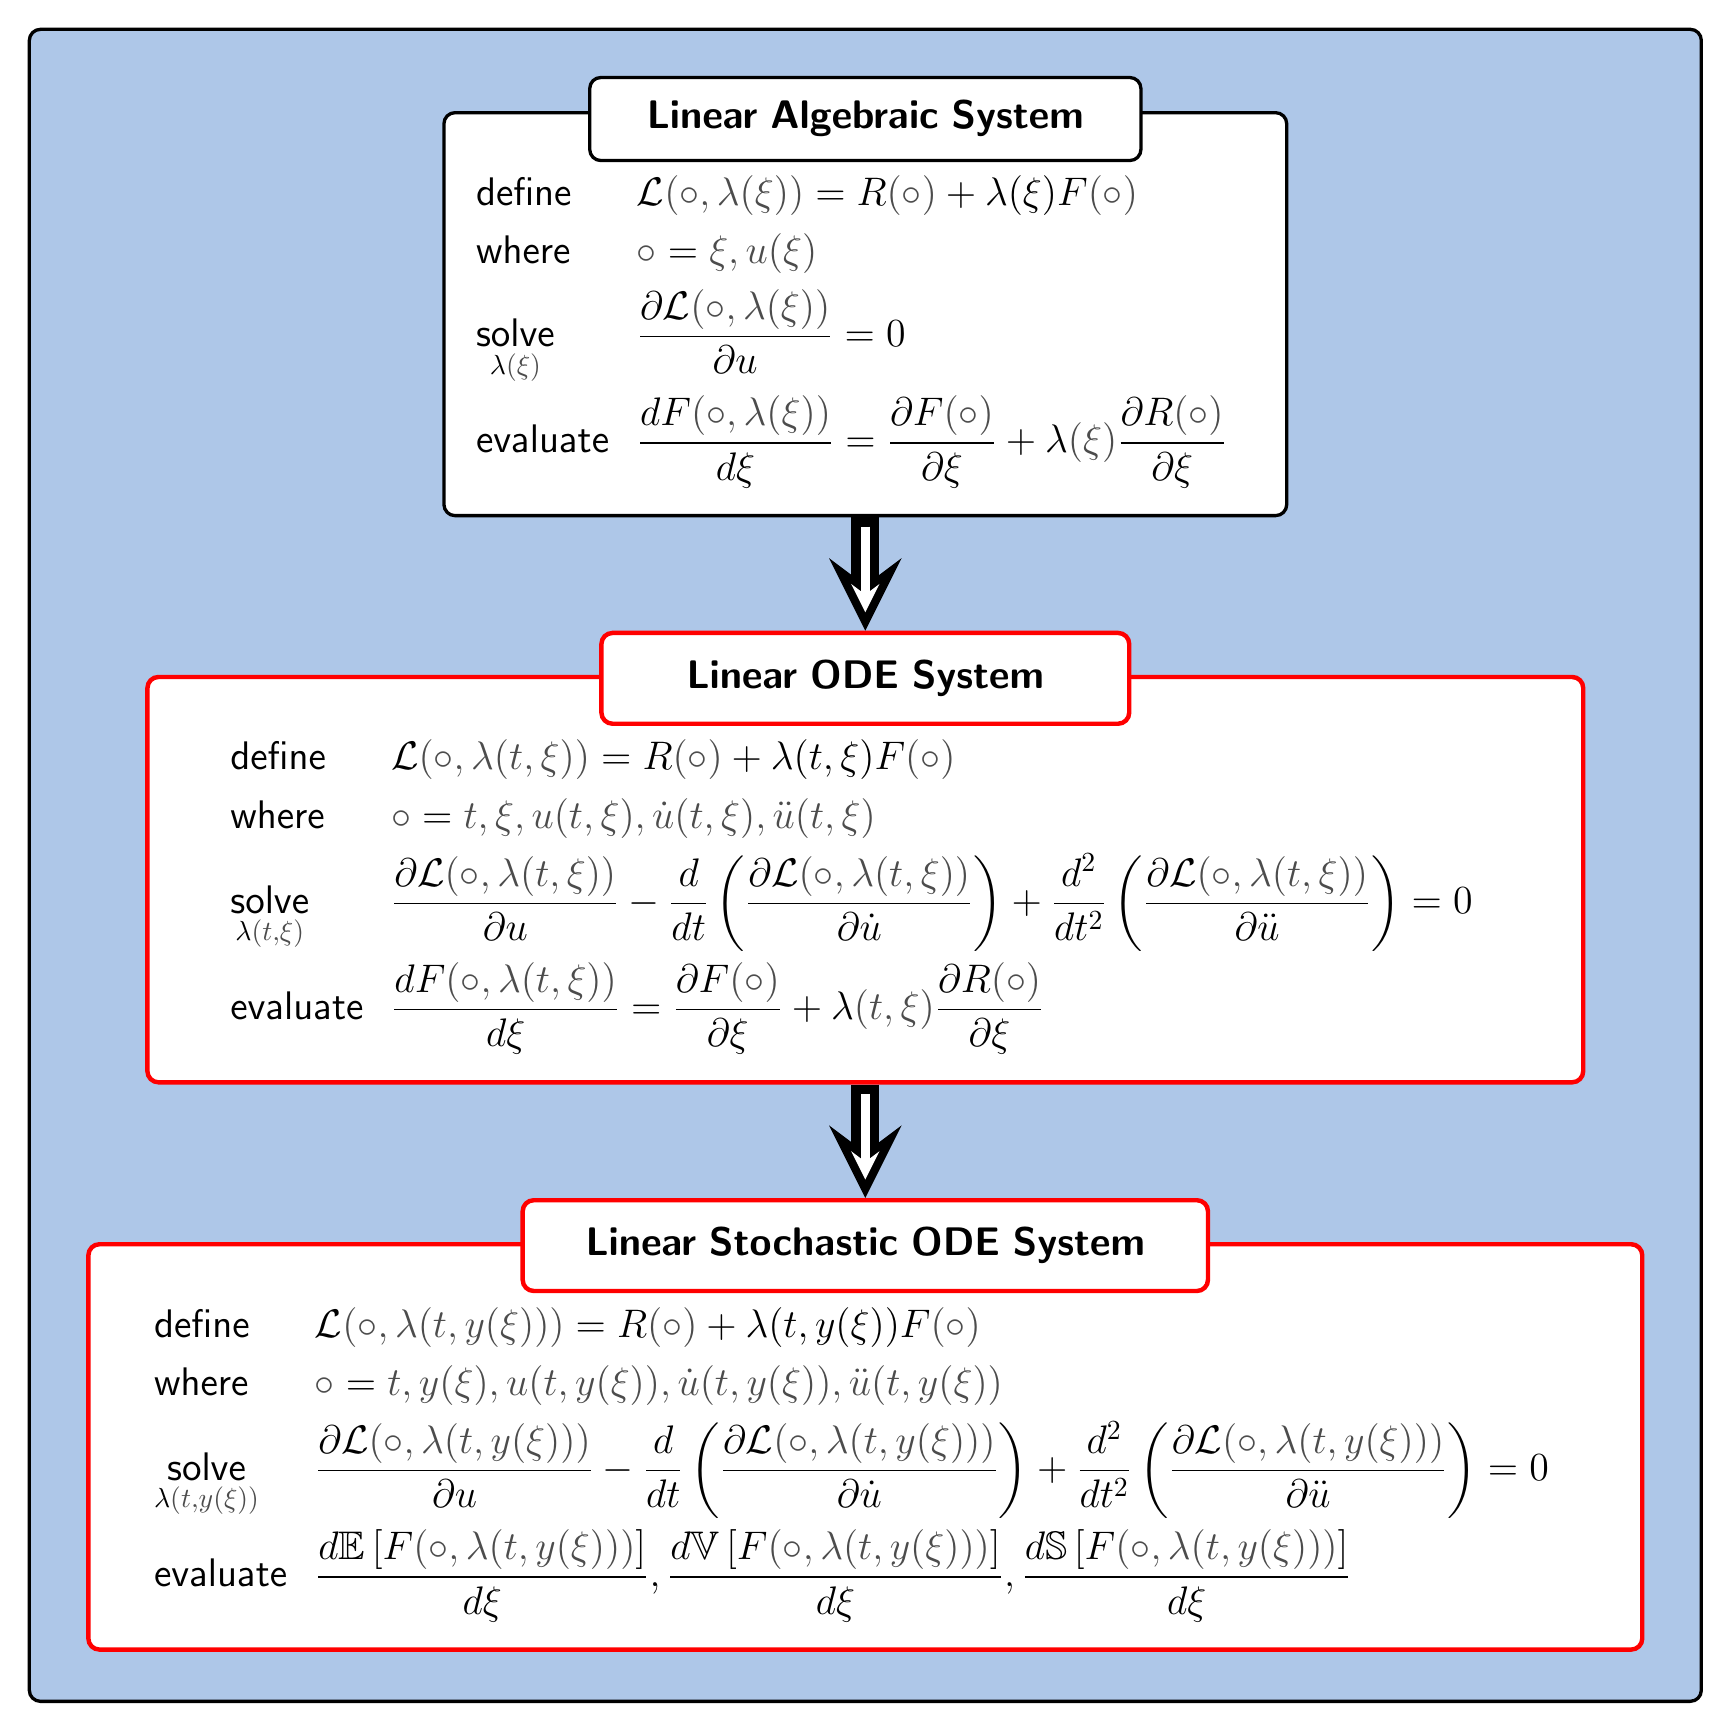
\begin{tikzpicture}

%  \node [block, very thick, node distance=3.5cm, text width=20cm, text height = 20cm, fill=lblue,font=\Large] (1) at (0,0) {};  

  \node [block, very thick, node distance=3.5cm, text width=21.cm, text height = 21cm, fill=lblue,font=\Large] (1) at (0,-7) {};  

  %%%%%%%%%%%%%%%%%%%%%%%%%%%%%%%%%%%%%%%%%%%%%%%%%%%%%%%%%%%%%%
  %                    NONLINEAR ALBEBRAIC SYSTEM              %
  %%%%%%%%%%%%%%%%%%%%%%%%%%%%%%%%%%%%%%%%%%%%%%%%%%%%%%%%%%%%%%
  
  \node [block, very thick, 
    node distance=5cm, 
    inner ysep=1em, 
    inner xsep=1em, 
    text width=10cm,
    fill=white!30,
    font=\Large] at (0,0) (static-physics) {
    \begin{equation}\nonumber
      \begin{aligned}
        & \text{define}                               &  & {\cal{L}}\arg{\carg{\circ},\lambda(\xi)} = {R}\arg{\carg{\circ}} + \lambda(\xi) {F}\arg{\carg{\circ}} & \\
        & \text{where}                                &  & \carg{\circ} = \sarg{\xi, u(\xi)}  & \\
        & \underset{\lambda\arg\xi}{\text{solve}} &  & \pd{\mathcal{L}\arg{\carg{\circ},\lambda(\xi)}}{u}  = 0 & \\
        & \text{evaluate}                         &  & \td{F\arg{\carg{\circ},\lambda(\xi)}}{\xi}  = \pd{F\arg{\carg{\circ}}}{\xi} + \lambda\arg\xi \pd{R\arg{\carg{\circ}}}{\xi} & \\
      \end{aligned}
    \end{equation}
  };
  \node [block, very thick, 
    node distance=0.0cm, 
    inner ysep=0em,
    inner xsep=0em, 
    text width=7cm,
    fill=white,
    font=\Large, above = -0.65cm of static-physics] (static-physics-header) {
    \textbf{Linear Algebraic System}
  };

  %%%%%%%%%%%%%%%%%%%%%%%%%%%%%%%%%%%%%%%%%%%%%%%%%%%%%%%%%%%%%%
  %                    NONLINEAR ODE                           %
  %%%%%%%%%%%%%%%%%%%%%%%%%%%%%%%%%%%%%%%%%%%%%%%%%%%%%%%%%%%%%% 
  
  \node [block, ultra thick, 
    node distance=4.75cm, 
    inner ysep=1em, 
    text width=18cm,
    fill=white!30,
    font=\Large, draw =red, below = 2cm of static-physics] (temporal-physics) {
    \begin{equation}\nonumber
      \begin{aligned}
        & \text{define}                               &  & {\cal{L}}\arg{\carg{\circ},\lambda(t,\xi)} = {R}\arg{\carg{\circ}} + \lambda(t,\xi) {F}\arg{\carg{\circ}} & \\
        & \text{where}                                &  & \carg{\circ} =   \sarg{t, \xi, u(t, \xi), \dot{u}(t,\xi), \ddot{u}(t,\xi)} & \\
        & \underset{\lambda\arg{t,\xi}}{\text{solve}} &  & \pd{{\cal{L}}\arg{\carg{\circ},\lambda(t,\xi)}}{{u}} - \td{}{t}  \left(\pd{{{\cal{L}}\arg{\carg{\circ},\lambda(t,\xi)}}}{{\dot{u}}} \right) + \tdt{}{t}  \left(\pd{{{\cal{L}}\arg{\carg{\circ},\lambda(t,\xi)}}}{{\ddot{u}}} \right) = 0 & \\
        & \text{evaluate}                         &  & \td{F\arg{\carg{\circ},\lambda(t,\xi)}}{\xi}  = \pd{F\arg{\carg{\circ}}}{\xi} + \lambda\arg{t,\xi} \pd{R\arg{\carg{\circ}}}{\xi} & \\
      \end{aligned}
    \end{equation}
  };
  \node [block, ultra thick, 
    node distance=0.0cm, 
    inner ysep=1em,
    inner xsep=1em, 
    text width=6cm,
    fill=white,
    draw =red, 
    font=\Large, above = -0.65cm of temporal-physics] (temporal-physics-header) {
    \textbf{Linear ODE System}
  };

  %%%%%%%%%%%%%%%%%%%%%%%%%%%%%%%%%%%%%%%%%%%%%%%%%%%%%%%%%%%%%%
  %                    NONLINEAR STO. ODE                      %
  %%%%%%%%%%%%%%%%%%%%%%%%%%%%%%%%%%%%%%%%%%%%%%%%%%%%%%%%%%%%%% 
  
  \node [block, ultra thick, 
    node distance=5.5cm, 
    inner ysep=1em, 
    text width=19.5cm,
    fill=white!30,
    draw =red, 
    font=\Large, below = 2cm of temporal-physics] (stochastic-temporal-physics) {
    \begin{equation}\nonumber
      \begin{aligned}
        & \text{define}                                  &  & {\cal{L}}\arg{\carg{\circ},\lambda(t,y(\xi))} = {R}\arg{\carg{\circ}} + \lambda(t,y(\xi)) {F}\arg{\carg{\circ}} & \\
        & \text{where}                                &  & \carg{\circ} =   \sarg{t, y(\xi), u(t, y(\xi)), \dot{u}(t,y(\xi)), \ddot{u}(t,y(\xi))} & \\
        & \underset{\lambda\arg{t,y(\xi)}}{\text{solve}} &  & \pd{{\cal{L}}\arg{\carg{\circ},\lambda(t,y(\xi))}}{{u}} - \td{}{t}  \left(\pd{{{\cal{L}}\arg{\carg{\circ},\lambda(t,y(\xi))}}}{{\dot{u}}} \right) + \tdt{}{t}  \left(\pd{{{\cal{L}}\arg{\carg{\circ},\lambda(t,y(\xi))}}}{{\ddot{u}}} \right) = 0 & \\
        & \text{evaluate}          &  & \td{\mathbb{E}\left[ F\arg{\circ,\lambda(t,y(\xi))} \right] }{\xi}, \td{ \mathbb{V}\left[ F\arg{\circ,\lambda(t,y(\xi))} \right] }{\xi} ,\td{ \mathbb{S}\left[ F\arg{\circ,\lambda(t,y(\xi))} \right] }{\xi}   & \\
%        &                          &  & \td{}{\xi} \mathbb{V}\left[ F\arg{t,y(\xi)}  \right]  & \\
%        &                          &  & \td{}{\xi} \mathbb{S}\left[ F\arg{t,y(\xi)}  \right]  & \\
      \end{aligned}
      %\arg{t,y(\xi),u(t,y(\xi)),\dot{u}(t,y(\xi)),\ddot{u}(t,y(\xi)),\lambda(t,y(\xi))}
    \end{equation}
  };
  \node [block, ultra thick, 
    node distance=0.0cm, 
    inner ysep=1em,
    inner xsep=1em, 
    text width=8cm,
    fill=white,
    draw =red, 
    font=\Large, above = -0.65cm of stochastic-temporal-physics] (stochastic-temporal-physics-header) {
    \textbf{Linear Stochastic ODE System}
  };

  \draw[double arrow=10pt colored by black and white!30, rounded corners] (static-physics) -- (temporal-physics-header);
  \draw[double arrow=10pt colored by black and white!30, rounded corners] (temporal-physics) -- (stochastic-temporal-physics-header);
  
\end{tikzpicture}

\end{document}

  \draw[double arrow=7pt colored by black and lime,rounded corners]
  (uq-ouu)  -| (se);
  \draw[double arrow=7pt colored by black and lime,rounded corners]
  (uq-ouu) -| (temporal-analysis);
  \draw[double arrow=7pt colored by black and red]
  (temporal-analysis) -- (1);
  \draw[double arrow=7pt colored by black and red]
  (sensitivity-analysis) -- (1);
\end{tikzpicture}
\end{document}
